\chapter{Tóm tắt và kế hoạch tương lai}

\section{Đánh giá nhiệm vụ}

Trong quá trình thực hiện đồ án chuyên ngành này, tôi đã đạt được các mục tiêu sau đây:

\begin{itemize}
	\item Xác định mục tiêu, những yêu cầu chức năng và phi chức năng, các bên liên quan của trang web.
	\item Thiết kế các lược đồ usecase, quy trình làm việc, lược đồ lớp, lược đồ tuần tự, cơ sở dữ liệu và hệ thống kiến trúc.
	\item Nghiên cứu và phân tích điểm mạnh, điểm yếu của các công nghệ phù hợp sẽ sử dụng trong đồ án chuyên ngành.
	\item Thiết kế giao diện người dùng, tạo khung dây cho các trang chính.
	\item Phân tích các trang web liên quan, so sánh và cải thiện đối với trang web của mình.
\end{itemize}
\newpage
Dưới đây là kế hoạch cho giai đoạn 1 của Đồ án chuyên ngành:

\begin{figure}[H]
	\centering
	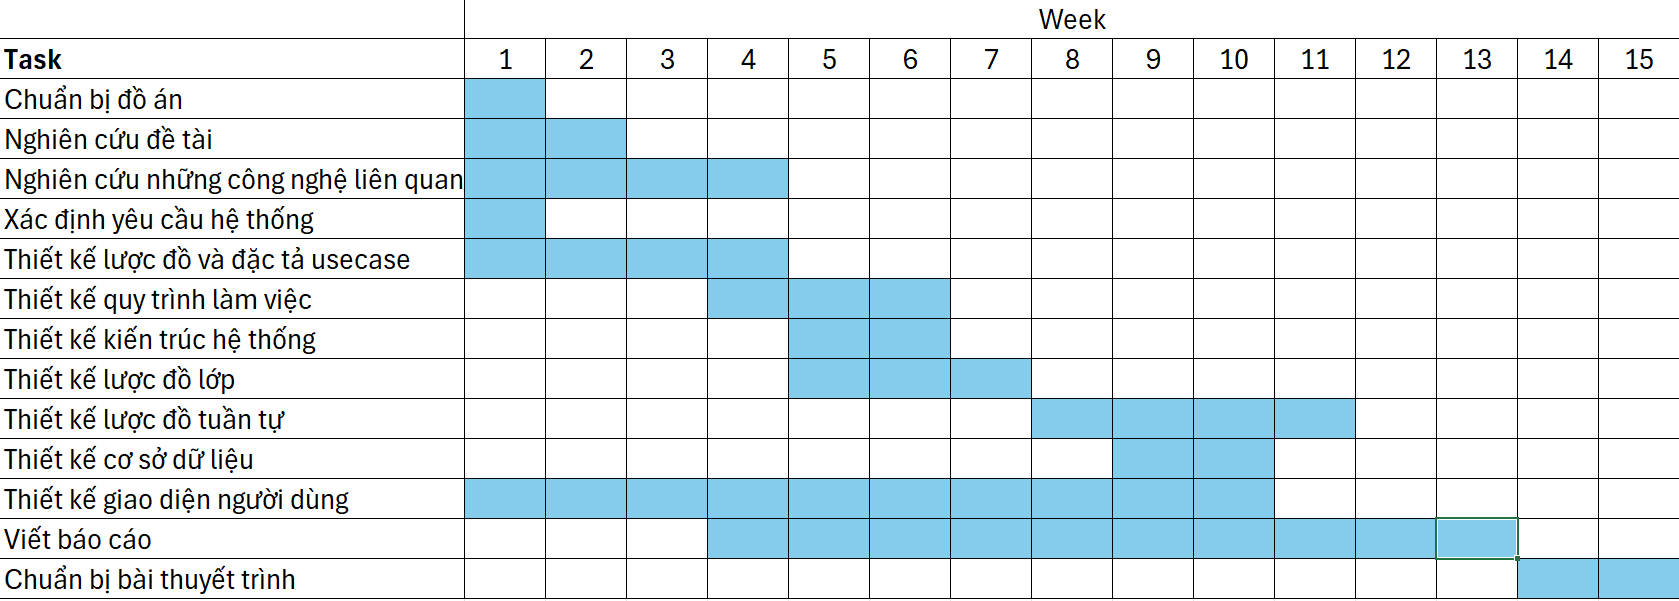
\includegraphics[scale=0.35]{img/TKB_GD1.png}
	\caption{Kế hoạch cho Giai đoạn 1 của Đồ án chuyên ngành}
\end{figure}


\section{Kế hoạch tương lai}

Trong giai đoạn tiếp theo, tôi có kế hoạch dự định hiện thực những chức năng sau:

\begin{itemize}
	\item Trong 2 tuần đầu, tôi sẽ thiết lập môi trường code và thư viện
	\item 4 tuần sau đó, tôi sẽ thiết kế sơ qua những giao diện người dùng đã được vẽ ở trên mà không sử dụng cơ sở dữ liệu.
	\item Vào tuần thứ 6 của đồ án, tôi sẽ nghiên cứu và xây dựng cơ sở dữ liệu cho trang web. Đến tuần thứ 7 sẽ thêm dữ liệu vào database và bắt đầu thử nghiệm thêm API vào trang web. Tuần 8, 9 và 10, tôi sẽ thử nghiệm và sửa lỗi của trang web. Và hoàn thiện những trang chính của trang web.
	\item Đồng thời, ở tuần 8, 9, 10 và 11, tôi nghiên cứu và hiện thức các chức năng liên quan đến CV như: nhập dữ liệu từ file PDF, trích xuất dữ liệu từ hệ thống thành file PDF.
	\item Việc kiếm nghiệm và sửa lỗi trang web sẽ được thực hiện xuyên suốt trong quá trình xây dựng trang web.
	\item Quá trình deploy sẽ được thực hiện ngay khi trang web đã hoàn tất.
\end{itemize}


Dưới đây là kế hoạch cho giai đoạn 2 của Đồ án tốt nghiệp:

\begin{figure}[H]
	\centering
	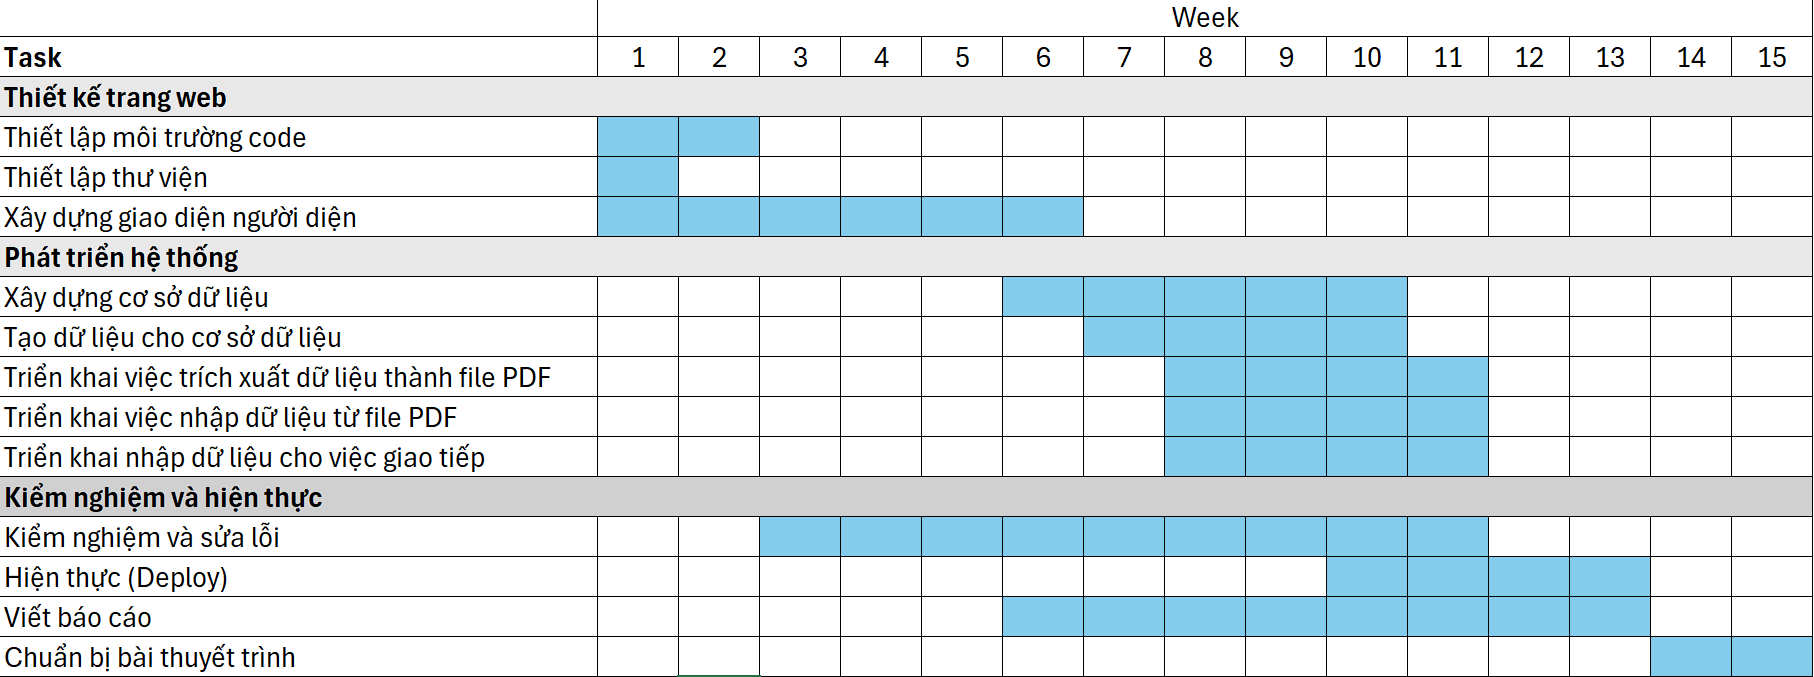
\includegraphics[scale=0.35]{img/TKB_GD2.png}
	\caption{Kế hoạch cho Giai đoạn 2 của Đồ án tốt nghiệp}
\end{figure}